\subsection{Управление программным средством}

\subsubsection{Вход в аккаунт}

Перед началом работы с программным средством пользователю необходимо авторизоваться в системе. Необходимо ввести логин, пароль и нажать
на кнопку отправки формы. Если данные валидны, то пользователя пропускают в систему, после чего можно ознакомится со всем функционалом
программного средства.

\subsubsection{Создание новой задачи}

Используя боковое меню в веб-приложении можно перемещаться между страницами программного средства. Выбрав там элемент «Новая задача»
пользователь может создать новую задачу. У задачи можно указывать приоритет, статус, участников и файлы.

\subsubsection{Просмотр всех задач}

Для просмотра всех задач можно использовать основную страницу приложения, где в виде интерактивной панели где задачи группированы по
приоритетам и статусам. 

На странице задач пользователя можно просмотреть все задачи в которых учавствует текущий пользователь. Информация отображается в виде 
таблицы со всей основной иформацией. Нажав на строку с задачей, пользователь может изучить задачу подробнее. Помимо страницы задач
пользователя существует страница всех задач на которой можно увидеть все задачи созданные в системе.

\subsubsection{Настройки приложения}

Особенностью программного средства является гибкая настройка внешнего вида. Пользователю доступны следующие настройки:
\begin{itemize}
    \item смена цветовой палитры;
    \item изменение положения навигационной панели;
    \item смена вспомогательного цвета блоков;
    \item изменение основного шрифта;
\end{itemize}

Внешний вид панели настроек показан на рисунке \ref{fig:settings}.

\begin{figure}[ht]
    \centering
    \fbox{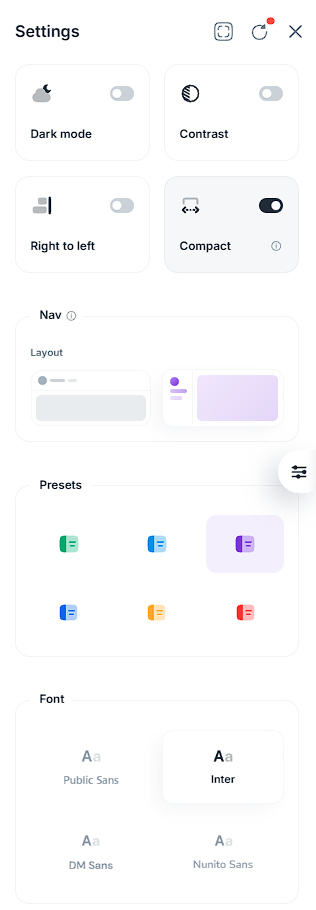
\includegraphics[width=0.35\linewidth]{\commonSecPathPrefix/sec_5/content/settings.png}}
    \caption{Панель настроек программного средства}
    \label{fig:settings}
\end{figure}

Также пользователь может изменить положение всех блоков, контраст и компактность. Дополнительно, можно открыть веб-приложение
в полноэкранном режиме.

Все настройки сохраняются у пользователя на устройстве, что помогает не запоминать настройки, а изменить их единожды и изменять при 
необходимости. Последний введённые логин и пароль пользователем также сохраняется на устройстве для подстановки в момент следующего
входа.